\section{Testing}

\subsection{Testing tools}

The Jmeter Testing tool was used during the testing part of the project. 

JMeter is a tool that helps to measure the performance of applications that are using HTTP protocol. It allows users to create their own test plans, which gives necessary flexibility for this project. Jmeter was configured in order to simulate JSON and HTML requests that are required to render single page. The Jmeter configuration is presented in Appendix B \ref{fig:jmeter_conf}. JMeter also builds the plot and the table of the request that was made with the corresponding time parameters.


\subsection{Performance Comparison of Redis and Web caches}

% describe jmeter configuration

During the project experiments with several configurations were conducted. The list of configurations is presented below:

\begin{itemize}
  \item Middleware server with Redis cache
  \item Middleware server with Varnish web cache
  \item Middleware server with Apache Traffic server cache
  \item Middleware server with HQL and second level cache
  \item Middleware server with HQL, second level cache and data compression
  \item Middleware server with HQL, second level cache and firs level cache
  \item Middleware server with HQL, second level cache, firs level cache and data compression
\end{itemize}

As can be seen, the tests are devided on two main parts: configurations for testing internal cache replacement and configurations for testing VMO creation. The first part analyzes and evaluates performance of redis cache and web cache servers. The second part  evaluates HVG performance. In the end the corresponding conclusion is made. 

Each experiment consists of several parts and can be described as an algorithm below: 

1. Configure Jmeter Test plan
2. Run Jmeter Test plan on predefined set of parallel request(which emulate users)
3. Evaluate Summary Report

For each test next configuration was used: Jmeter emulates one hundred users that are making ten continuous requests for fetching the view model object of the main page.  


\subsection{Performance evaluation of Redis Cache and CDN}

This type of test emulates the user requests for generating view model object for maing page. In order to build a VMO several requests should be done for gathering data model objects. The request for building single page consists of nine REST subrequests through HTTP protocol for gatheing DMOs.  The corresponding Jmeter test plan is presented on figure [TODO: Add figure].


\begin{figure}[h]
    \centering
    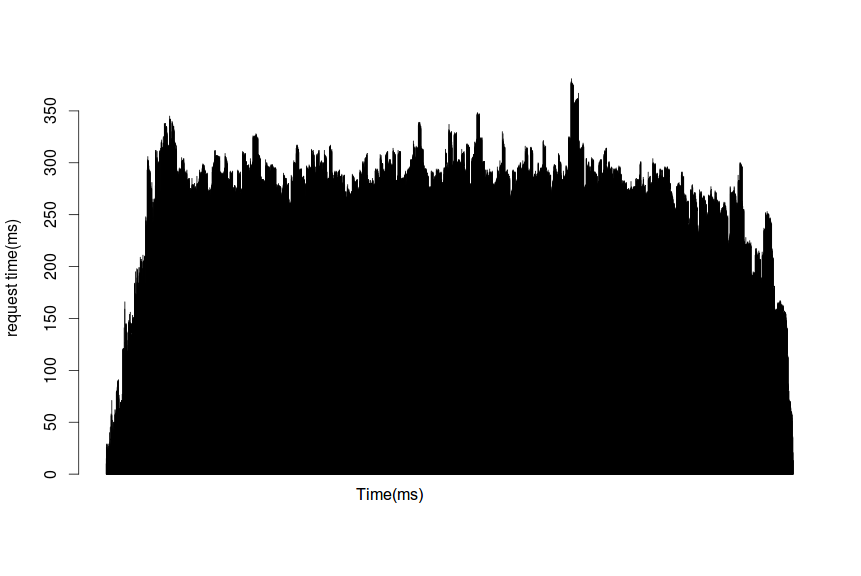
\includegraphics[width=\textwidth]{images/vmo_redis_mult_par.png}
    \caption{Response time of middleware server wihth Redis cache for generating VMO through parallel requests}
    \label{fig:vmo_redis_mult_par}
\end{figure}

Figure \ref{fig:vmo_redis_mult_par} illustrates server response time for generating VMO that has no dependencies between objects. As can be seen, the maximum response time is about 300 ms. Figure \ref{fig:vmo_redis_mult_seq} shows response time from middleware server for generating hierarchical VMO that tree structure is shown on [TODO: add]. This VMO is generated by executing three sequential requests for coresponding data model objects. As can be seen the performance decreases about three times. It is quite predictable because it is necessary to make three sequential requests. Figure \ref{fig:vmo_varnish_mult} shows the VMO generation through Varnish web cache. As can be seen, the response time decreases dramatically. The reason of that is that it takes constant time for getting data from Varnish web cache. The request for getting DMO rarely touches the middleware server. It is noticable from the figure, when the request goes through varnish web cache to the middleware server the response time increases. Figure \ref{fig:vmo_ts_mult} shows the response time for making requests through Apache Traffic server configured as a web cache. The results more predictable than the results of varnish web cache. Theh maximum time does not reach 100 ms.  


\begin{figure}[h]
    \centering
    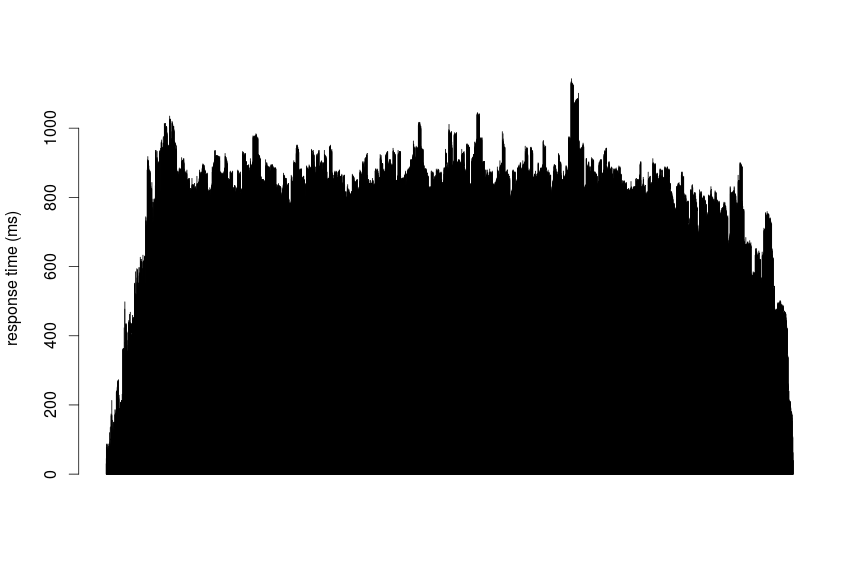
\includegraphics[width=\textwidth]{images/vmo_redis_mult_seq.png}
    \caption{Response time of middleware server wihth Redis cache for generating hierarchical VMO through sequential requests}
    \label{fig:vmo_redis_mult_seq}
\end{figure}


\begin{figure}[h]
    \centering
    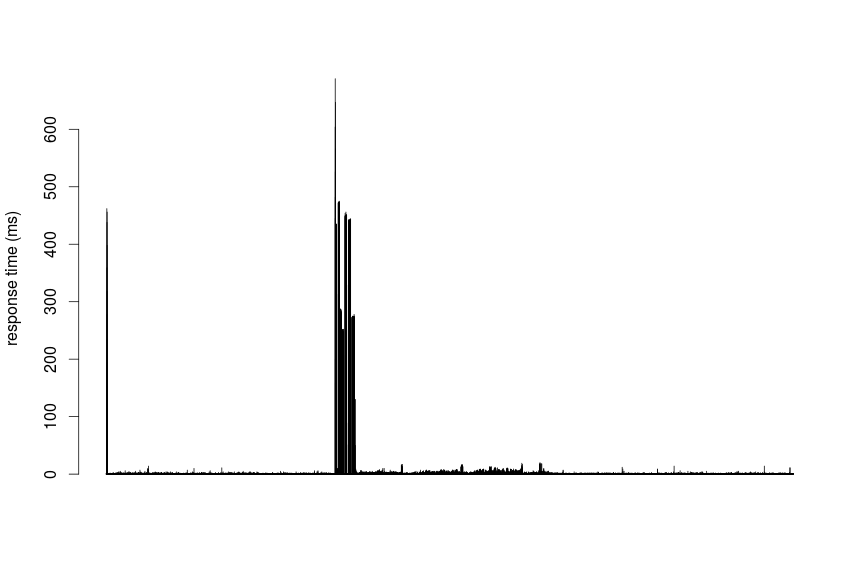
\includegraphics[width=\textwidth]{images/vmo_varnish_mult.png}
    \caption{Response time of Varnish web cache for generating hierarchical VMO}
    \label{fig:vmo_varnish_mult}
\end{figure}


\begin{figure}[h]
    \centering
    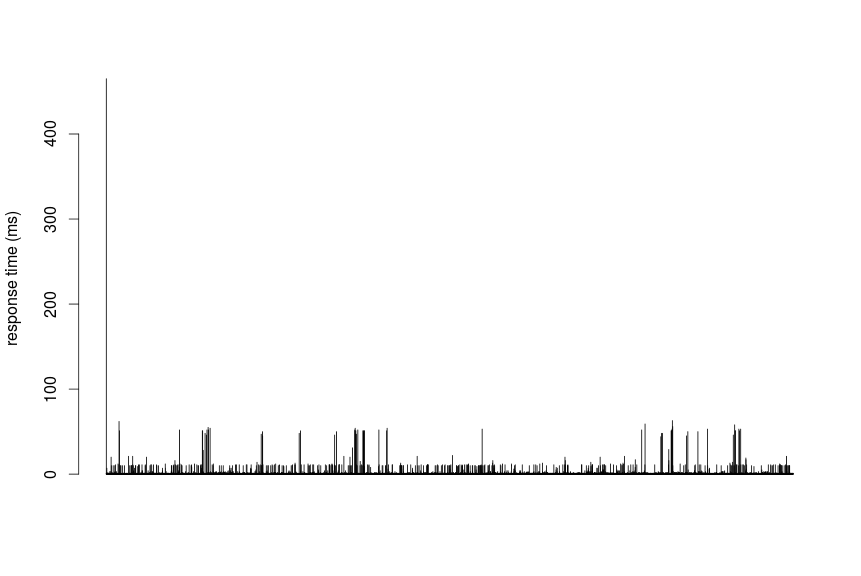
\includegraphics[width=\textwidth]{images/vmo_ts_mult.png}
    \caption{Response time of Apache Traffic Server for generating hierarchical VMO}
    \label{fig:vmo_ts_mult}
\end{figure}

Figure \ref{fig:vmo_hvg} shows the response time for hierarchical VMO generator with different configurations. As can be seen, there are four hills, each hill represents the corresponding experiment: HVG with first level cache(caching data model objects), HVG with first level cache and data compression, HVG with first and second level caches(caching both data model objects and view model objects) and HVG with first and second level cache and data compression. The first hill appears to be the slowest one, responses come in around 6000ms in the worst case. The behaviour is quite unpredictable, because the vmo requests consume 100\% of CPU and the amount of data that is transferred between client and middleware server is quite big. The summary report on [TODO: add summary report] shows execution staistic.

The second hill amost twice faster than the first one. The reason of that is the reduced amount of data transferred between client and server. The compression reduces amount of data almost in five times. As can be seen, the compression does not produce overhead and slows responses for a negligable(?) time. In addition, the hill looks more predictable and has no big [vpadin??].  

The third hill shows the response time from middleware server with two level caches. As can be seen, the server performance three times faster than the hill number two and almost six times faster than the first hill. This happens because the middleware server executes requests for building VMOs rearely, and checks if VMO is already computed every time before executing actuall request. 

The last hill presents the response time with second and first level caches and data compression. It can be noticed, that the hill is more stable than the third one, but the execution time roughly the same.

The brief result is that the optimal configuration for HVG is two level cache and data compression.

\begin{figure}[h]
    \centering
    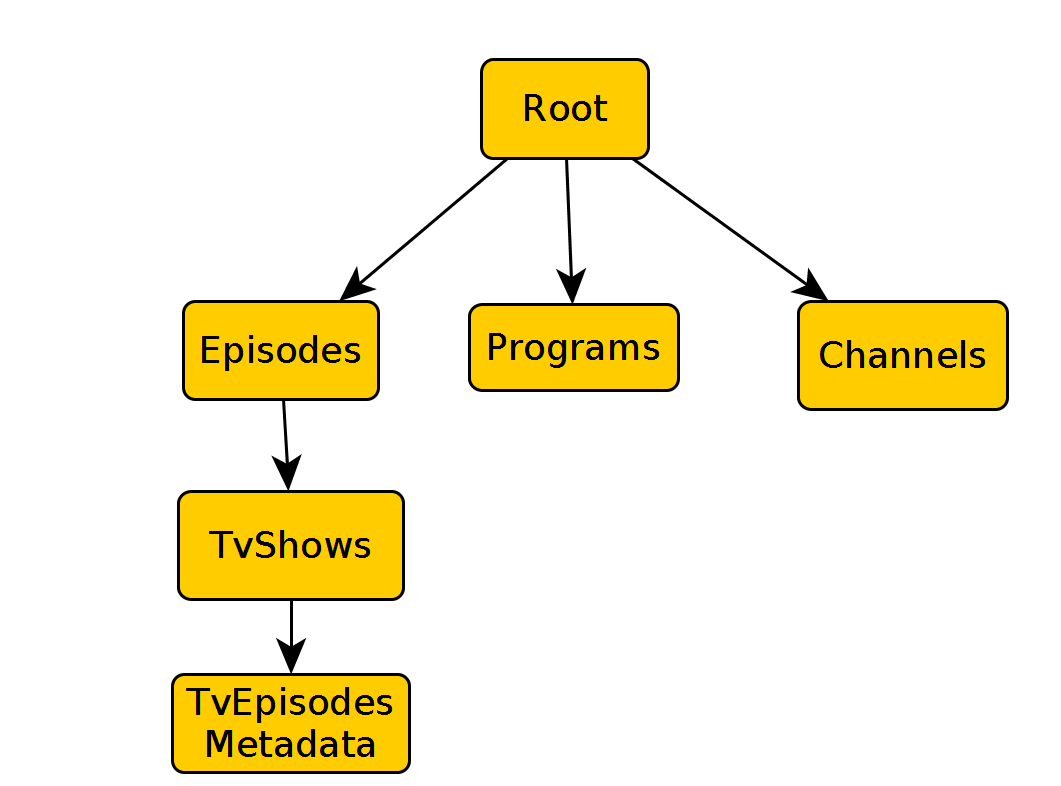
\includegraphics[width=\textwidth]{images/vmo_test_example.png}
    \caption{View Model Object that is used during testing}
    \label{fig:vmo_test_example}
\end{figure}



\begin{figure}[h]
    \centering
    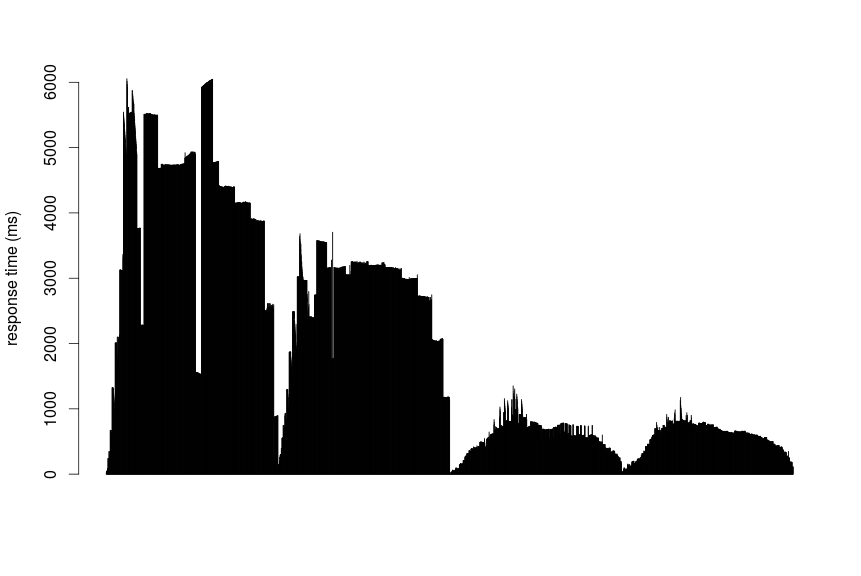
\includegraphics[width=\textwidth]{images/vmo_hvg.png}
    \caption{Response time of middleware server for generating hierarchical VMO through HVG}
    \label{fig:vmo_hvg}
\end{figure}

Figure \ref{fig:hvg_loadtest} demonstrates the load test for optimal HVG configuration. During the test around 50000(fifty thousand) request was made in one hundred parallel threads. There are two peaks can be observed that have response time around 10.000 msec. During these requests, the middleware server requested data from the underlying content distributor. There can be seen that the mean response time is around ~1500 msec.


\begin{figure}[h]
    \centering
    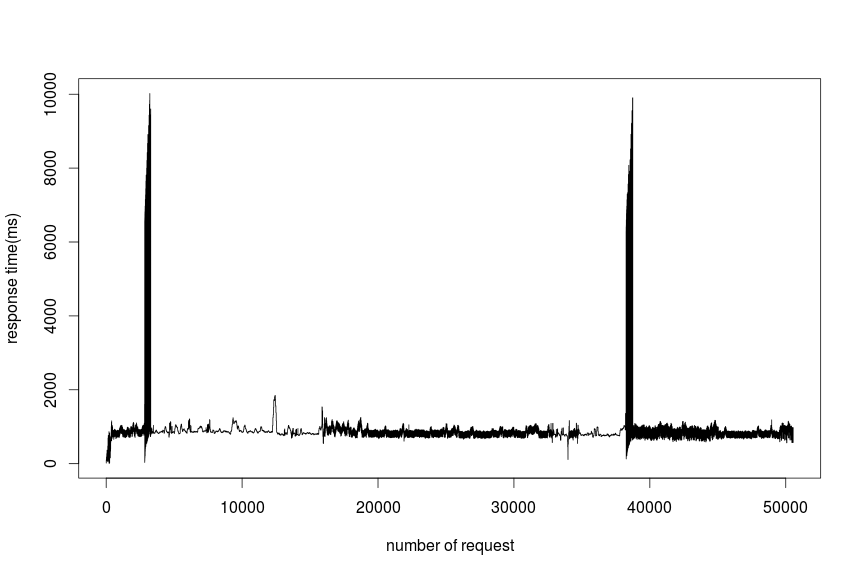
\includegraphics[width=\textwidth]{images/hql_loadtest.png}
    \caption{Load test of optimal HVG configuration}
    \label{fig:hvg_loadtest}
\end{figure}

The tests executed up until this point were conducted without introducing latency. The next obvious step is to make an artificial latency and observe how the server response time depends on it. The artificial latency is about ~500 msec between client and server. Figure \ref{fig:hvg_comparison} shows the comparison between responses with artificial latency and without. As can be seen there is one big peak on the green plot, is appeared because several events appeared at the same time: the data in the redis cache became stale and the redis server could not write data fast enough due to lack of resources. The red plot also has one peak, the reason of it is the stale data in redis cache and corresponding request to the content provider.


\begin{figure}[h]
    \centering
    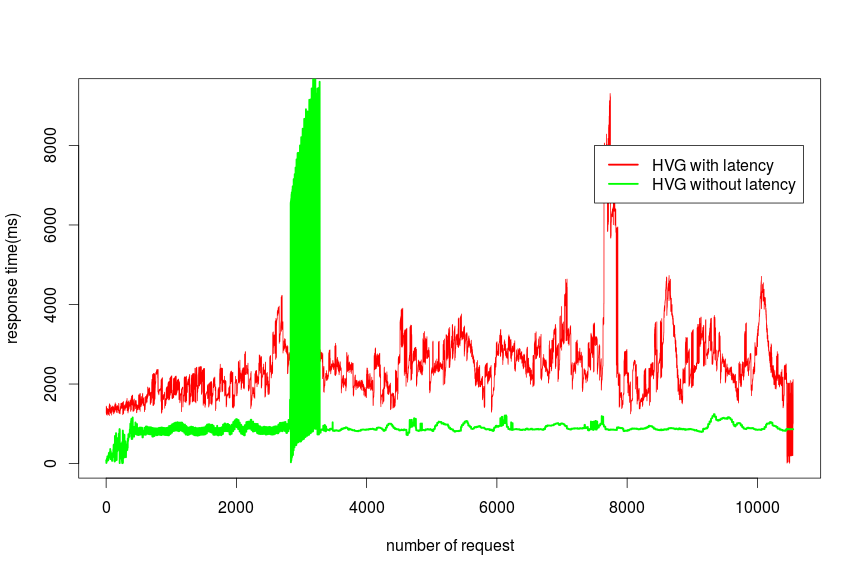
\includegraphics[width=\textwidth]{images/hvg_latency_comparison.png}
    \caption{Comparison of response time with and without latency for optimal HVG configuration}
    \label{fig:hvg_comparison}
\end{figure}

The next figure \ref{fig:vmo_comparison} shows the comparison between responses with and without latency for generating VMO through multiple requests. There can be observed that the server made several responses to the content distributor as a result the request time is about ~6000 msec. In some cases the response time for requests with latency less than the response time without latency. It is a small persentage of errors during the experimets. When these errors occur, the server sends immediately empty response.


\begin{figure}[h]
    \centering
    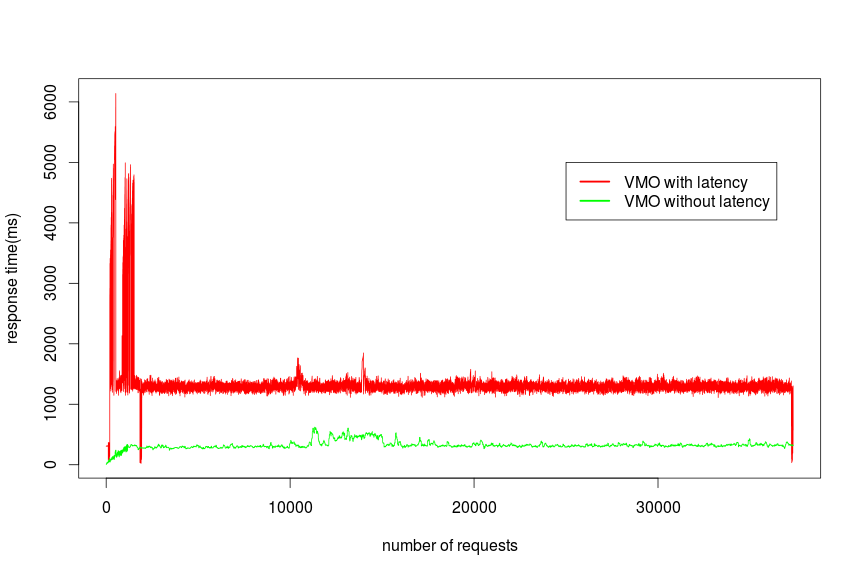
\includegraphics[width=\textwidth]{images/vmo_parallel_comparison.png}
    \caption{Comparison of response time with and without latency for VMO generation without dependencies using multiple requests}
    \label{fig:vmo_comparison}
\end{figure}


Figure \ref{fig:hvg_vmo_latency_comp} shows the comparison between HVG with optimal configuration and VMO generated through multiple requests. As can be seen during the HVG test the several requests were made to the content distributor. The red plot also shows that the VMO through multiple requests also did several requests because of the stale content. Both plots had a small error during the experiment, as a result server responses with approximately ~10 ms can be observed. The HVG with optimal configuration shows great performance comparing to the VMO through multiple requests. In addition, it is more stable and reliable. 

\begin{figure}[h]
    \centering
    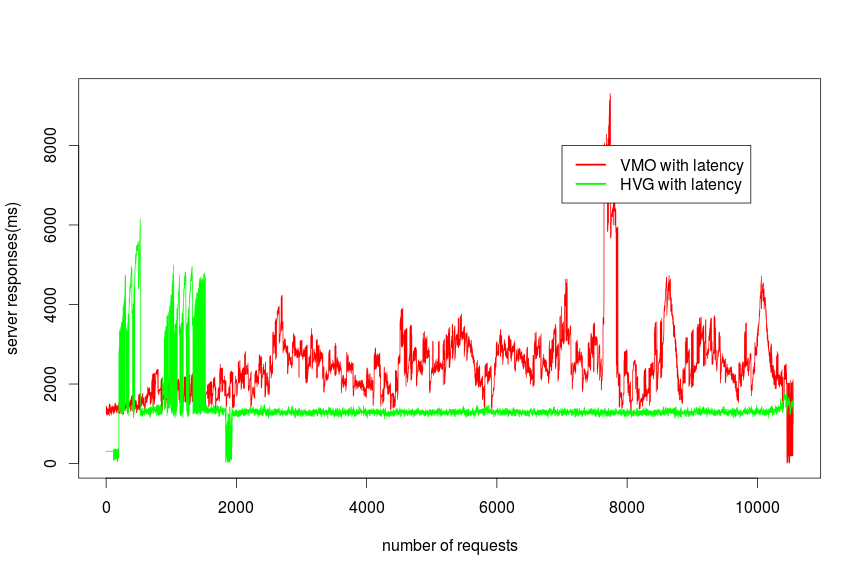
\includegraphics[width=\textwidth]{images/hvg_vmo_latency_comparison.png}
    \caption{Comparison of response time between parallel VMO generation and HVG with optimal configuration}
    \label{fig:hvg_vmo_latency_comp}
\end{figure}


\subsection{Performance evaluation of HVG with different configurations}


\subsection{Comparion of Redis cache, CDN and HVG solutions}


\subsection{Testing frameworks}



% Use cases for requests: (selection of the optimal request/response headers for the dynamic and static contents)
% 1. LastModified and If-Modified-Since
% 2. Cache-Control: s-maxage, (public, private?, must-revalidate)
% 3. Etag and If-None-Match
% 4. Combination: Etag + LastModified
% 5. Combination: Etag + LastModified + CacheControl


\newpage



% The summary report field exlanation is presented in table \ref{table:jmeter_summary}. 

% % \begin{table}
% %   \begin{itemize}
% %     \item Label  -- The name of the script that was executed
% %     \item Samles -- The amount of responses that was executed
% %     \item Average -- The average response time, represented in milliseconds
% %     \item Min -- the minimum time for the response 
% %     \item Max -- the maximum time for the response
% %     \item Std. Dev.  -- standard deviation from the average response time
% %     \item Error -- the persentage of error responses
% %     \item Throughput -- the throughput represented in responses per second
% %     \item KB/sec -- the data transferred per second
% %     \item Avg. Bytes -- the amount of bytes transferred per response
% %   \end{itemize}
% %   \label{table:jmeter_summary}
% % \end{table}
